\documentclass{article}
\usepackage[a4paper, margin=2cm]{geometry}
\usepackage{xcolor}
\usepackage{xspace}
\usepackage{booktabs}
\usepackage{dsfont}
\usepackage{footmisc}
\usepackage{marvosym}
\usepackage{amsmath}
\usepackage{hyperref}
\usepackage[capitalise,noabbrev]{cleveref}
\usepackage{tabularx}
\usepackage{listings}
\usepackage{multirow}
\usepackage{pgfplots}
\pgfplotsset{compat=newest}

\usepgfplotslibrary{groupplots}
\pgfplotsset{every axis/.style={scale only axis}}

\pgfplotsset{
  % Mark repeat, but the last mark is always drawn
  mark repeat*/.style={
    scatter,
    scatter src=x,
    scatter/@pre marker code/.code={
      \pgfmathtruncatemacro\usemark{
        or(mod(\coordindex,#1)==0, (\coordindex==(\numcoords-1))
      }
      \ifnum\usemark=0
        \pgfplotsset{mark=none}
      \fi
    },
    scatter/@post marker code/.code={}
  },
  log x ticks with fixed point/.style={
      xticklabel={
        \pgfkeys{/pgf/fpu=true}
        \pgfmathparse{exp(\tick)}%
        \pgfmathprintnumber[fixed relative, precision=3]{\pgfmathresult}
        \pgfkeys{/pgf/fpu=false}
      }
  },
  log y ticks with fixed point/.style={
      yticklabel={
        \pgfkeys{/pgf/fpu=true}
        \pgfmathparse{exp(\tick)}%
        \pgfmathprintnumber[fixed relative, precision=3]{\pgfmathresult}
        \pgfkeys{/pgf/fpu=false}
      }
  },
  major grid style={thin,dotted},
  minor grid style={thin,dotted},
  ymajorgrids,
  yminorgrids,
  every axis/.append style={
    line width=0.7pt,
    tick style={
      line cap=round,
      thin,
      major tick length=4pt,
      minor tick length=2pt,
    },
    mark options={solid},
  },
  legend cell align=left,
  legend style={
    line width=0.7pt,
    /tikz/every even column/.append style={column sep=3mm,black},
    /tikz/every odd column/.append style={black},
    mark options={solid},
  },
  % move title closer
  legend style={font=\small},
  title style={yshift=-2pt},
  % less space on left and right
  enlarge x limits=0.04,
  every tick label/.append style={font=\footnotesize},
  every axis label/.append style={font=\small},
  every axis y label/.append style={yshift=-1ex},
  /pgf/number format/1000 sep={},
  axis lines*=left,
  xlabel near ticks,
  ylabel near ticks,
  axis lines*=left,
  label style={font=\footnotesize},
  tick label style={font=\footnotesize},
  width=65mm,
  height=55mm,
  log x ticks with fixed point,
}

\definecolor{veryLightGrey}{HTML}{F2F2F2}
\definecolor{lightGrey}{HTML}{DDDDDD}
\definecolor{colorSimdRecSplit}{HTML}{444444}
\definecolor{colorChd}{HTML}{377EB8}
\definecolor{colorRustFmph}{HTML}{A65628}
\definecolor{colorRustFmphGo}{HTML}{A65628}
\definecolor{colorRustPHast}{HTML}{FF5733}
\definecolor{colorSicHash}{HTML}{4DAF4A}
\definecolor{colorPthash}{HTML}{984EA3}
\definecolor{colorDensePtHash}{HTML}{377EB8}
\definecolor{colorRecSplit}{HTML}{FF7F00}
\definecolor{colorBbhash}{HTML}{F781BF}
\definecolor{colorShockHash}{HTML}{F8BA01}
\definecolor{colorBipartiteShockHash}{HTML}{F781BF}
\definecolor{colorBipartiteShockHashFlat}{HTML}{E41A1C}
\definecolor{colorBmz}{HTML}{000000}
\definecolor{colorBdz}{HTML}{444444}
\definecolor{colorFch}{HTML}{444444}
\definecolor{colorChm}{HTML}{A65628}
\definecolor{colorFiPS}{HTML}{FF7F00}

\newlength{\squareWidth}
\newlength{\squareHeight}
\setlength{\squareWidth}{1.0\pgfplotmarksize}
\setlength{\squareHeight}{1.3\pgfplotmarksize}
\pgfdeclareplotmark{heatmapSquare}{%
  \pgfpathmoveto{\pgfqpoint{ \squareWidth}{ \squareHeight}}%
  \pgfpathlineto{\pgfqpoint{ \squareWidth}{-\squareHeight}}%
  \pgfpathlineto{\pgfqpoint{-\squareWidth}{-\squareHeight}}%
  \pgfpathlineto{\pgfqpoint{-\squareWidth}{ \squareHeight}}%
  \pgfpathclose%
  \pgfusepath{fill}
}

\title{MPHF plot}
\date{}
\begin{document}

% IMPORT-DATA competitorNames _competitorNames.txt

% IMPORT-DATA paretoConstruction dominance-map.txt
% SQL DELETE FROM paretoConstruction WHERE threads != 1 OR loadFactor != 1.0
% SQL DELETE FROM paretoConstruction WHERE name = "PartitionedPTHash" OR name = "Consensus"
% SQL DELETE FROM paretoConstruction WHERE constructionTimeMilliseconds > 5000000
%% SQL DELETE FROM paretoConstruction
%% WHERE EXISTS (SELECT * FROM paretoConstruction d WHERE paretoConstruction.name = d.name
%%             AND d.bitsPerElement < paretoConstruction.bitsPerElement
%%             AND d.constructionTimeMilliseconds < paretoConstruction.constructionTimeMilliseconds)

% IMPORT-DATA paretoQuery dominance-map.txt
% SQL DELETE FROM paretoQuery WHERE threads != 1 OR loadFactor != 1.0
% SQL DELETE FROM paretoQuery WHERE name = "PartitionedPTHash" OR name = "Consensus"
% SQL DELETE FROM paretoQuery WHERE constructionTimeMilliseconds > 5000000
%% SQL DELETE FROM paretoQuery
%% WHERE EXISTS (SELECT * FROM paretoQuery d WHERE paretoQuery.name = d.name
%%             AND d.bitsPerElement < paretoQuery.bitsPerElement
%%             AND d.queryTimeMilliseconds < paretoQuery.queryTimeMilliseconds)

% IMPORT-DATA pareto dominance-map.txt
% SQL DELETE FROM pareto WHERE threads != 1 OR loadFactor != 1.0
% SQL DELETE FROM pareto WHERE name = "PartitionedPTHash" OR name = "Consensus"

% SQL CREATE TABLE valuesForQueryThroughput (sampleQueryThroughput INT)
% SQL INSERT INTO valuesForQueryThroughput VALUES (1),(2),(3),(4),(5),(6),(7),(8),(9),(10),(11),(12),(13),(14),(15),(16),(17),(18),(19),(20),(21),(22),(23),(24),(25),(26),(27),(28),(29),(30),(31),(32),(33),(34),(35),(36),(37),(38),(39),(40),(41),(42),(43),(44),(45)
% SQL CREATE TABLE valuesForConstructionThroughput (sampleConstructionThroughput INT)
% SQL INSERT INTO valuesForConstructionThroughput VALUES(0.5),(1),(1.5),(2),(2.5),(3),(3.5),(4),(4.5),(5),(5.5),(6),(6.5),(7),(7.5),(8),(8.5),(9),(9.5),(10),(10.5),(11),(11.5),(12),(12.5),(13),(13.5),(14),(14.5),(15),(15.5),(16),(16.5),(17),(17.5),(18),(18.5),(19),(19.5),(20),(20.5),(21),(21.5),(22),(22.5),(23),(23.5),(24) 
% SQL CREATE TABLE valuesForSpace (sampleSpace INT)
% SQL INSERT INTO valuesForSpace VALUES(0.00),(0.05),(0.10),(0.15),(0.20),(0.25),(0.30),(0.35),(0.40),(0.45),(0.50),(0.55),(0.60),(0.65),(0.70),(0.75),(0.80),(0.85),(0.90),(0.95),(1.00),(1.05),(1.10),(1.15),(1.20),(1.25),(1.30),(1.35),(1.40),(1.45),(1.50),(1.55),(1.60),(1.65),(1.70),(1.75),(1.80),(1.85),(1.90),(1.95),(2.00) 

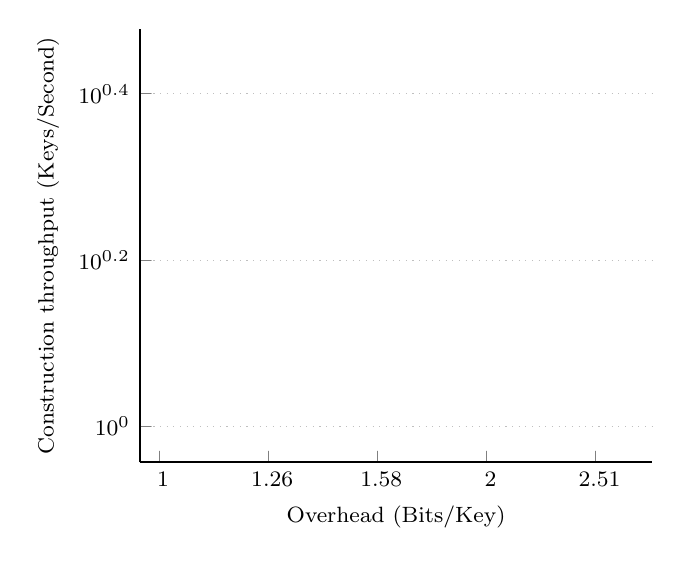
\begin{tikzpicture}
    \begin{axis}[
            ylabel={Construction throughput (Keys/Second)},
            xlabel={Overhead (Bits/Key)},
            xmode=log,
            ymode=log,
            legend columns=4,
            legend to name=legend,
        ]
        %% MULTIPLOT(name|ptitle|attr)
        %% SELECT
        %%    bitsPerElement-1.4427 as x,
        %%    1000.0*N/constructionTimeMilliseconds as y,
        %%    store_attr || IIF(name LIKE "%PTHash" OR name LIKE "%SicHash" OR name LIKE "ShockHash%", ",mark repeat*=4", "") as attr,
        %%    IFNULL(store_name, "name" || "-> NOT IN JOIN") as ptitle,
        %%    MULTIPLOT
        %% FROM paretoConstruction scatterplot
        %% LEFT JOIN competitorNames ON name = store_code
        %% ORDER BY store_name,x,y
    \end{axis}
\end{tikzpicture}
%
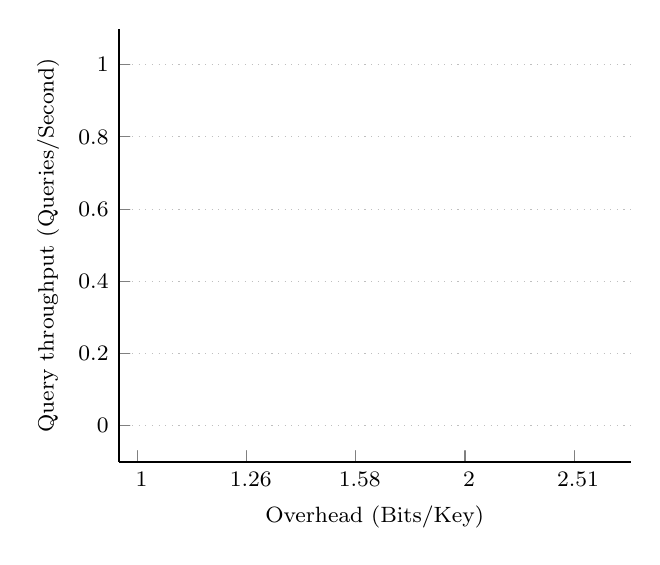
\begin{tikzpicture}
    \begin{axis}[
            ylabel={Query throughput (Queries/Second)},
            xlabel={Overhead (Bits/Key)},
            legend columns=2,
            xmode=log,
        ]
        %% MULTIPLOT(name|ptitle|attr)
        %% SELECT
        %%    bitsPerElement-1.4427 as x,
        %%    1000.0*numQueries/queryTimeMilliseconds as y,
        %%    store_attr as attr,
        %%    IFNULL(store_name, "name" || "-> NOT IN JOIN") as ptitle,
        %%    MULTIPLOT
        %% FROM paretoQuery scatterplot
        %% LEFT JOIN competitorNames ON name = store_code
        %% ORDER BY store_name,x,y

        \legend{}
    \end{axis}
\end{tikzpicture}

\setlength{\squareWidth}{1.55\pgfplotmarksize}
\setlength{\squareHeight}{0.75\pgfplotmarksize}
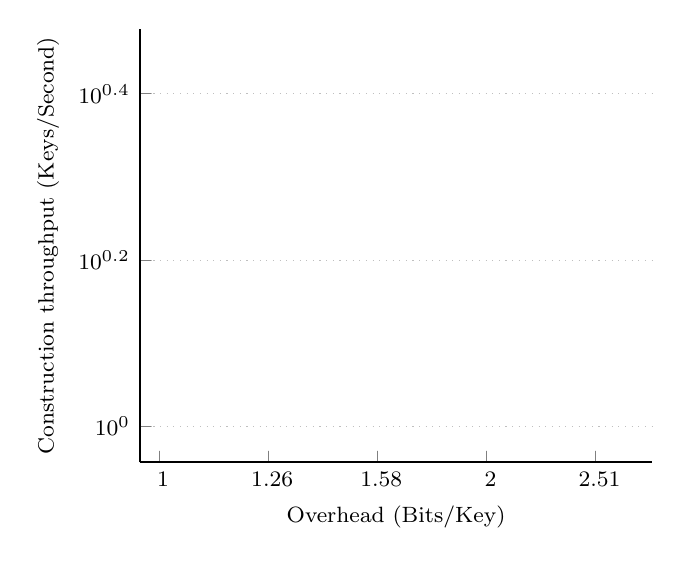
\begin{tikzpicture}
    \begin{axis}[
            ylabel={Construction throughput (Keys/Second)},
            xlabel={Overhead (Bits/Key)},
            only marks,
            xmode=log,
            ymode=log,
        ]
        %% MULTIPLOT(ptitle|ptitle|attr)
        %% SELECT
        %%    pow(2.0, 3.5*sampleSpace-6) AS x,
        %%    1000000.0*pow(2.0, 0.4*sampleConstructionThroughput-5) AS y,
        %%    (SELECT name FROM pareto o WHERE o.bitsPerElement-1.4427 <= pow(2.0, 3.5*sampleSpace-6) AND 0.001*o.N/o.constructionTimeMilliseconds >= pow(2.0, 0.4*sampleConstructionThroughput-5) ORDER BY queryTimeMilliseconds ASC LIMIT 1) AS best,
        %%    store_attr || ",mark=heatmapSquare" as attr,
        %%    IFNULL(store_name, "name" || "-> NOT IN JOIN") as ptitle
        %% FROM valuesForConstructionThroughput
        %% CROSS JOIN valuesForSpace
        %% LEFT JOIN competitorNames ON best=store_code
        %% WHERE best IS NOT NULL
        %% ORDER BY store_name,x,y

        % Markers:
        %% MULTIPLOT(ptitle|ptitle|attr)
        %% SELECT
        %%    AVG(pow(2.0, 3.5*sampleSpace-6))      + IIF(store_code=="ShockHashSIMD", -0.01, IIF(store_code=="BipartiteShockHash", +0.01, IIF(store_code=="SIMDRecSplit", -0.08, 0))) AS x,
        %%    1000000.0*(AVG(pow(2.0, 0.4*sampleConstructionThroughput-5)) + IIF(store_code=="ShockHashSIMD",     0, IIF(store_code=="BipartiteShockHash", -0.09, IIF(store_code=="SIMDRecSplit", -0.01, 0)))) AS y,
        %%    (SELECT name FROM pareto o WHERE o.bitsPerElement-1.46 <= pow(2.0, 3.5*sampleSpace-6) AND 0.001*o.N/o.constructionTimeMilliseconds >= pow(2.0, 0.4*sampleConstructionThroughput-5) ORDER BY queryTimeMilliseconds ASC LIMIT 1) AS best,
        %%    store_attr || ",color=white" || IIF(store_code="ShockHashSIMD", ",mark options={scale=1.2}", "") || IIF(store_code="DensePartitionedPTHash", ",mark=phobicInverse", "") || IIF(store_code="FiPS", ",mark=fingerprintInverse", "") || IIF(store_code="ShockHashSIMD", ",mark=shockhashInverse", "") as attr,
        %%    store_name as ptitle
        %% FROM valuesForConstructionThroughput
        %% CROSS JOIN valuesForSpace
        %% LEFT JOIN competitorNames ON best=store_code
        %% WHERE best IS NOT NULL
        %% GROUP BY store_name
        %% ORDER BY store_name,x,y

        \legend{}
    \end{axis}
\end{tikzpicture}
%
\setlength{\squareWidth}{1.45\pgfplotmarksize}
\setlength{\squareHeight}{0.75\pgfplotmarksize}
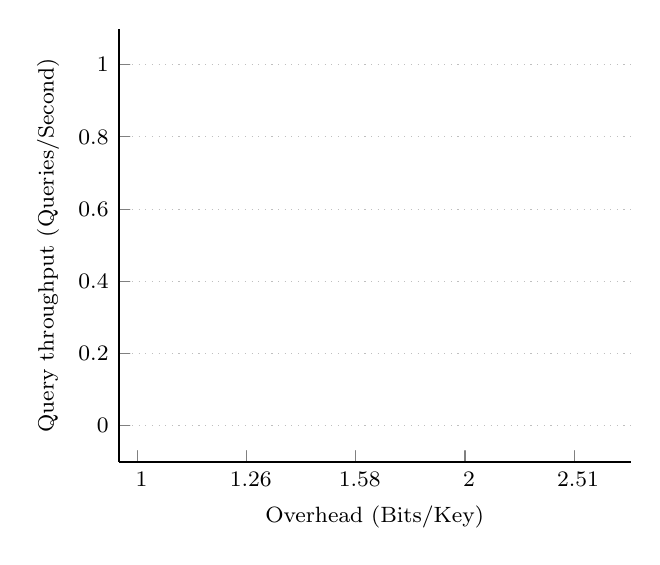
\begin{tikzpicture}
    \begin{axis}[
            ylabel={Query throughput (Queries/Second)},
            xlabel={Overhead (Bits/Key)},
            legend columns=4,
            only marks,
            xmode=log,
        ]
        %% MULTIPLOT(ptitle|ptitle|attr)
        %% SELECT
        %%    pow(2.0, 3.5*sampleSpace-6) AS x,
        %%    1000000.0*sampleQueryThroughput AS y,
        %%    (SELECT name FROM pareto o WHERE o.bitsPerElement-1.4427 <= pow(2.0, 3.5*sampleSpace-6) AND 0.001*o.numQueries/o.queryTimeMilliseconds >= sampleQueryThroughput ORDER BY constructionTimeMilliseconds ASC LIMIT 1) AS best,
        %%    store_attr || ",mark=heatmapSquare" as attr,
        %%    IFNULL(store_name, "name" || "-> NOT IN JOIN") as ptitle
        %% FROM valuesForQueryThroughput
        %% CROSS JOIN valuesForSpace
        %% LEFT JOIN competitorNames ON best=store_code
        %% WHERE best IS NOT NULL
        %% ORDER BY store_name,x,y

        % Markers:
        %% MULTIPLOT(ptitle|ptitle|attr)
        %% SELECT
        %%    AVG(pow(2.0, 3.5*sampleSpace-6)) + IIF(store_code=="BipartiteShockHash", -0.01, IIF(store_code=="ShockHashSIMD", -0.00, IIF(store_code=="PTHash", 0, 0))) AS x,
        %%    1000000.0*(AVG(sampleQueryThroughput)       + IIF(store_code=="BipartiteShockHash",     0, IIF(store_code=="ShockHashSIMD",     0, IIF(store_code=="PTHash", 2, 0)))) AS y,
        %%    (SELECT name FROM pareto o WHERE o.bitsPerElement-1.46 <= pow(2.0, 3.5*sampleSpace-6) AND 0.001*o.numQueries/o.queryTimeMilliseconds >= sampleQueryThroughput ORDER BY constructionTimeMilliseconds ASC LIMIT 1) AS best,
        %%    store_attr || ",color=white" || IIF(store_code="ShockHashSIMD", ",mark options={scale=1.2}", "") || IIF(store_code="DensePartitionedPTHash", ",mark=phobicInverse", "") || IIF(store_code="FiPS", ",mark=fingerprintInverse", "") || IIF(store_code="ShockHashSIMD", ",mark=shockhashInverse", "") as attr,
        %%    store_name as ptitle
        %% FROM valuesForQueryThroughput
        %% CROSS JOIN valuesForSpace
        %% LEFT JOIN competitorNames ON best=store_code
        %% WHERE best IS NOT NULL
        %% GROUP BY store_name
        %% ORDER BY store_name,x,y

        \legend{}
    \end{axis}
\end{tikzpicture}

\centering
\begin{tikzpicture}
    \ref*{legend}
\end{tikzpicture}

\end{document}

